\paragraph{QuizziPedia::Front-End::Services::QuizService}
\begin{figure}[ht]
	\centering
	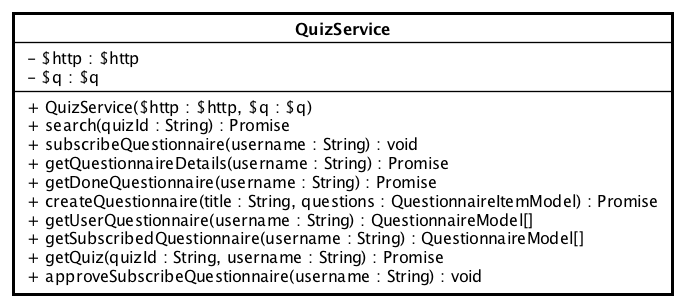
\includegraphics[scale=0.80]{UML/Classi/Front-End/QuizziPedia_Front-end_Services_QuizService.png}
	\caption{QuizziPedia::Front-End::Services::QuizService}
\end{figure}\FloatBarrier
\begin{itemize}
	\item \textbf{Descrizione}: questa classe permette di ottenere i dati di un quiz tramite delle parole chiave inserite dall'utente nella barra di ricerca. Permette inoltre di iscriversi ad un questionario e di scaricare l'intera lista di domande di un questionario a partire dal suo id univoco;
	\item \textbf{Utilizzo}: fornisce le funzionalità per ottenere i dati di un quiz in seguito ad una ricerca dell'utente, passando i risultati ai controllers. Ritorna dei riferimenti alle domande del quiz;
	\item \textbf{Relazione con altre classi:}
	\begin{itemize}
		\item \textit{IN} \texttt{QuestionnaireModel}: rappresenta un questionario. Contiene tutte le informazioni necessarie alla
		presentazione del contenuto del questionario; 
		\item \textit{OUT} \texttt{SearchController}: questa classe permette di gestire la ricerca di questionari e utenti all'interno dell'applicazione;
		\item \textit{OUT} \texttt{QuestionsController}: questa classe permette di gestire il recupero delle domande per poterle stampare nella modalità allenamento;
		\item \textit{OUT} \texttt{QuestionnaireDetailsController}: questa classe permette di gestire i dettagli di un questionario;
		\item \textit{OUT} \texttt{FillingQuestionnaireController}: questa classe permette di gestire la compilazione del questionario;
		\item \textit{OUT} \texttt{CreateQuestionnaireController}: questa classe permette di gestire la creazione di un questionario;
		\item \textit{OUT} \texttt{RegistrationManagementController}: questa classe permette di gestire le iscrizione degli utenti ai questionari;
		\item \textit{OUT} \texttt{ResultsController}: questa classe permette di gestire le iscrizione degli utenti ai questionari; 
		\item \textit{OUT} \texttt{QuestionnaireManagementController}: questa classe permette di gestire tutti i questionari creati da un utente. 
		
	\end{itemize}
	\item \textbf{Attributi:}
	\begin{itemize}
		\item \texttt{-} \texttt{\$http: \$http} \\ Campo dati che contiene un riferimento al servizio \$http che permette la comunicazione con il protocollo \textit{HTTP\ped{G}};
		\item \texttt{-} \texttt{\$q: \$q} \\ Campo dati che contiene un riferimento a \$q, un servizio offerto da \textit{AngularJS\ped{G}} per la gestione, tramite \textit{Promise\ped{G}}, di chiamate asincrone.
	\end{itemize}
	\item \textbf{Metodi:} 
	\begin{itemize}
		\item \texttt{+} \texttt{QuizService(\$http: \$http, \$q: \$q)} \\ Metodo costruttore della classe. \\
		\textbf{Parametri}:
		\begin{itemize}
			\item \texttt{\$http: \$http} \\ Campo dati che contiene un riferimento al servizio \$http che permette la comunicazione con il protocollo \textit{HTTP\ped{G}};
			\item \texttt{\$q: \$q} \\ Campo dati che contiene un riferimento a \$q, un servizio offerto da \textit{AngularJS\ped{G}} per la gestione, tramite \textit{Promise\ped{G}}, di chiamate asincrone. 
		\end{itemize}
	\item \texttt{+} \texttt{search(quizId: String): Promise} \\Metodo che serve per recuperare i questionari dopo averne selezionato uno dalla lista ottenuta da una ricerca. Il metodo ritorna una \textit{Promise\ped{G}}. In caso la \textit{Promise\ped{G}} venga rifiutata, verrà restituito al \texttt{SearchController} un oggetto \texttt{ErrorModelInfo} contenente tutti i dettagli dell'errore. In caso la \textit{Promise\ped{G}} venga accettata, verrà restituito al chiamante del metodo il risultato della chiamata.\\
	\textbf{Parametri}:
	\begin{itemize}
		\item \texttt{quizId: String} \\ Parametro che rappresenta il questionario da cercare.
	\end{itemize}
	\item \texttt{+} \texttt{subscribeQuestionnaire(quizId: String, username: String): Void} \\Metodo per iscriversi ad un questionario;
	\begin{itemize}
		\item \texttt{quizId: String} \\ Parametro che rappresenta il questionario in cui iscrivere l'utente;
		\item \texttt{username: String} \\ Parametro che rappresenta l'utente da registrare al questionario.
	\end{itemize}
	\item \texttt{+} \texttt{getQuestionnaireDetails(username: String): Promise} \\Metodo che serve per ritornare i dettagli di tutti i questionari creati da un utente; Il metodo ritorna una \textit{Promise\ped{G}}. In caso la \textit{Promise\ped{G}} venga rifiutata, verrà restituito al \texttt{StatisticsController} un oggetto \texttt{ErrorModelInfo} contenente tutti i dettagli dell'errore. In caso la \textit{Promise\ped{G}} venga accettata, verrà restituito al chiamante del metodo il risultato della chiamata.\\ 
     \textbf{Parametri}:
	\begin{itemize}
		\item \texttt{username: String} \\ Parametro che rappresenta l'utente del quale andranno caricati tutti i questionari.
	\end{itemize}
	\item \texttt{+ getDoneQuestionnaire(username: String): Promise} \\ Metodo che restituisce tutti i questionari svolti da un utente. Il metodo ritorna una \textit{Promise\ped{G}}. In caso la \textit{Promise\ped{G}} venga rifiutata, verrà restituito al \texttt{UserDetailsController} un oggetto \texttt{ErrorModelInfo} contenente tutti i dettagli dell'errore. \\
	\textbf{Parametri}: 
	\begin{itemize}
		\item \texttt{username: String} \\ Parametro che rappresenta l'utente del quale andranno caricati tutti i questionari svolti.
	\end{itemize}
	\item \texttt{+ createQuestionnaire(title: String, questions: QuestionnaireItemModel): Promise} \\ Metodo che permette di creare un nuovo questionario. Il metodo ritorna una \textit{Promise\ped{G}}. In caso la \textit{Promise\ped{G}} venga rifiutata, verrà restituito al \texttt{CreateQuestionnaireController} un oggetto \texttt{ErrorModelInfo} contenente tutti i dettagli dell'errore. In caso la \textit{Promise\ped{G}} venga accettata, verrà restituito al chiamante del metodo il risultato della chiamata.\\
	\textbf{Parametri}:
	\begin{itemize}
		\item \texttt{title: String} \\ Parametro che rappresenta il titolo del questionario.
		\item \texttt{questions: QuestionnaireItemModel} \\ Parametro contenente tutte le domande del questionario.
	\end{itemize}
	\item \texttt{+} \texttt{getUserQuestionnaire(username: String): QuestionnaireModel[]} \\Metodo che ritorna un array di QuestionnaireModel che sono tutti i questionari creati dall'utente in input.\\
	\textbf{Parametri}:
	\begin{itemize}
		\item \texttt{username: String} \\ Parametro che indica l'identificativo dell'utente del quale vogliamo richiedere i questionari.
	\end{itemize}
	\item \texttt{+} \texttt{getSubscribedQuestionnaire(username: String): QuestionnaireModel[]}: \\Metodo che ritorna la lista dei questionari a cui l'utente è iscritto.\\
	\textbf{Parametri}:
	\begin{itemize}
		\item \texttt{username: String} \\ Parametro che indica l'utente del quale scaricare i quiz a cui risulta iscritto.
	\end{itemize}
	\item \texttt{+ subscribeQuestionnaire(username: String): void} \\ Metodo che approva l'iscrizione di un determinato utente ad un quesitonario.
	\textbf{Parametri}:
	\begin{itemize}
		\item \texttt{username: String} \\ Parametro che indica l'utente da abilitare ad un questionario.
	\end{itemize}
	\item \texttt{getUserForThisQuestionnaire(quizId: String): Array} \\ Metodo che ritorna tutti gli utenti che hanno eseguito il questionario.
	\textbf{Parametri}:
	\begin{itemize}
		\item \texttt{quizId: String} \\ Paramentro che indica il questionario del quale scaricare gli utenti.
	\end{itemize}
	\item \texttt{+ getQuizResults(quizId: String): Object} \\ Metodo che ritorna i risultati di un questionario.
	\textbf{Parametri}:
	\begin{itemize}
		\item \texttt{quiId: String} \\ Id del questionario del quale recuperare i risultati.
	\end{itemize}
	\item \texttt{+ getQuiz(quizId: String, username: String): Promise} \\ Metodo che ritorna una \textit{Promise\ped{G}}. In caso la \textit{Promise\ped{G}} venga rifiutata, verrà restituito al \texttt{CreateQuestionnaireController} un oggetto \texttt{ErrorModelInfo} contenente tutti i dettagli dell'errore. In caso la \textit{Promise\ped{G}} venga accettata, cioè se l'utente è registrato, verrà restituito al chiamante il questionario. \\
	\textbf{Parametri}:
	\begin{itemize}
		\item \texttt{quiId: String} \\ Id del questionario del quale recuperare i risultati.
	\end{itemize}
\end{itemize}
\end{itemize}